\chapter{分组并行求解算法及其应用}\label{ch03}
在微分方程的求解中, 许多方法最终都能归结于代数方程组的求解. 这些求解方法的主要困难在于最终的代数方程组规模过大, 无法在有限的时间内求解. 为了解决这个问题, 本文首先提出了一种分组并行的求解算法, 并将其实现为 PGSolve 软件包. 然后, 本文以求$n$-孤子和1-LUMP相互作用解的直接代数方法为例, 展示了 PGSolve 对于大规模代数方程组的求解能力. 

\section{分组并行求解算法与PGSolve软件包}
代数方程组的求解是符号计算的核心问题之一. 尤其是多项式代数方程组的求解, 更是符号计算中最基础也是最困难的问题. 多项式代数方程组的求解算法有吴文俊先生的吴方法\cite{wu1984,wu1985}\D 正则列方法\cite{kalkbrener1991three,lu1994searching}和\Grobner{}基方法\cite{adams1994introduction}等. 吴方法的实现有王东明的charsets\cite{wang1995implementation}等. 正则列方法的实现有 RegularChains \cite{maza2000triangular}, 该软件包已经被包含在 Maple 的内置函数中. 求\Grobner{}基的相关算法有 Buchberger 算法\cite{buchberger1970algorithmic}\D F4 算法\cite{faugere1999new} 和 F5 算法\cite{faugere2002new}等. Maple 和 Mathematica 等计算机代数系统的内置求解函数都是以\Grobner{}基方法为基础实现的, 且\Grobner{}基方法不仅能够求解多项式方程组, 还能求解更加一般的代数方程组. 

上述方法的基本原理是将原方程组转化一个或多个三角化的方程组后在逐个求解, 且三角化后的方程组和原方程同解. 但是, 算法关于方程规模的时间复杂度都是指数的, 并且计算过程中表达式的中间结果膨胀十分严重, 难以在有限的时间和内存条件下求解大规模的方程组. 并且, 上述算法注重数学上的严谨性, 致力于求解原方程组所有的解. 然而在实际求解过程中, 我们往往只需要一部分的解, 这些算法解的完整性反而成为了降低求解效率的重要原因. 

因此, 为了高效地从大规模的代数方程组解的用户想要的解, 本文基于如下几点想法, 提出了一个分组并行的代数方程组求解算法.
\begin{compactenum}[(1)]
\item 对原方程组进行合理的分组后依次求解, 完成一个分组的求解后, 将解代入剩余的方程中继续求解. 
\item 在求解过程中删除不满足用户要求的解, 以减少解的分支, 提高求解效率.
\item 在适当的步骤中采用并行策略进行加速, 充分利用多核计算机的性能.
\end{compactenum}

\subsection{核心框架}
\begin{figure}[htbp]
\centering 
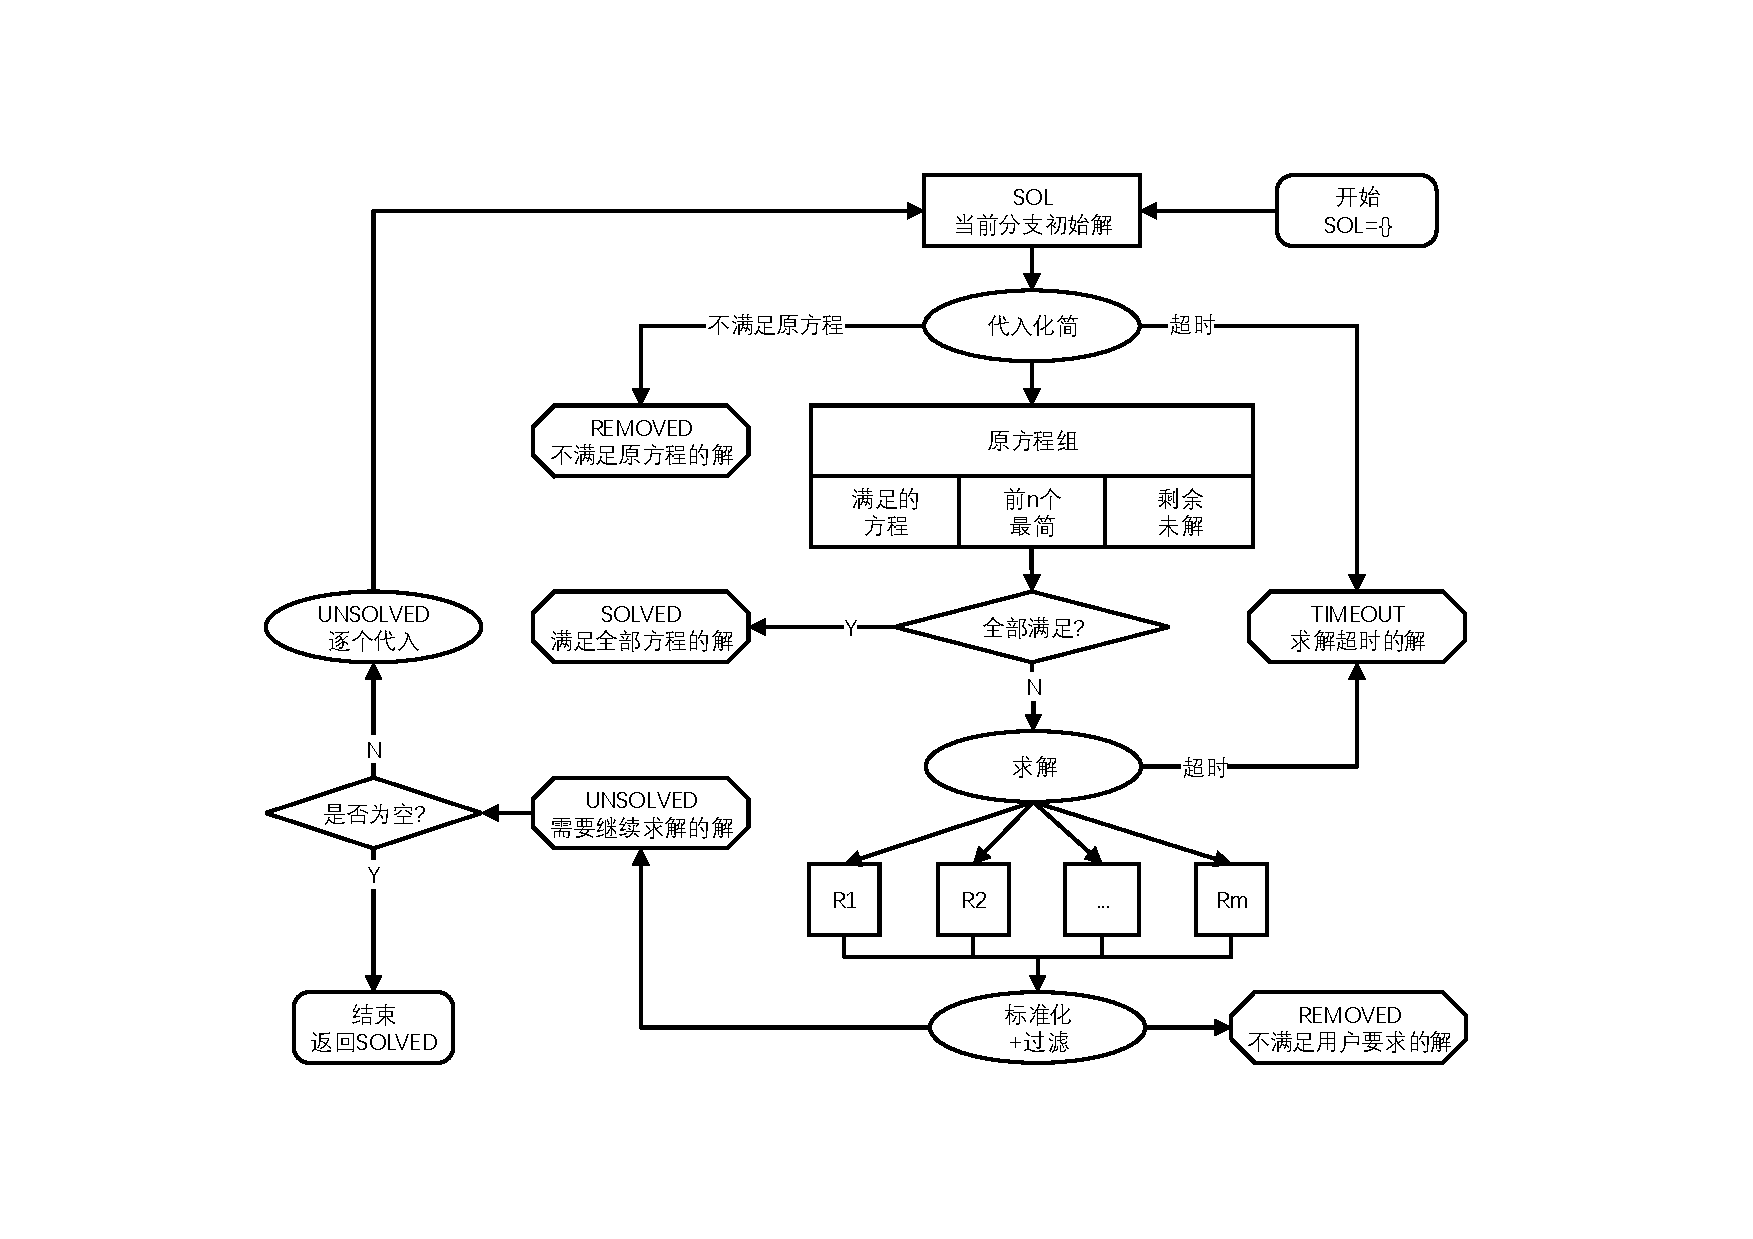
\includegraphics[width=0.9\textwidth]{fig/pgsolve.pdf}
\caption{PGSolve 算法框架}\label{PGSolve}
\end{figure}

根据上文的讨论, 本文设计如\reffig{PGSolve}所示的算法框架. 该算法的具体步骤如下:
\begin{compactenum}[Step 1.]
\item 初始化: 用于保存解集的 SOLVED\D UNSOLVED 以及 TIMEOUT 三个容器为空集. 令 SOL=\{\}. 
\item 将当前解SOL代入原方程组之后并化简. 化简之后, 原方程组可以分为三个部分. 第一部分是已经满足的方程, 这些方程在代入化简后为零. 将剩余的方程按照复杂度进行升序排序之后, 可以根据用户给定的n分为两个部分. 
\item 在代入化简后, 
    \begin{compactenum}[(a)]
    \item 如果存在一些方程的化简结果为常数, 则表示SOL不满足原方程组, 我们将其废弃后进入下一个分支的求解. 
    \item 若SOL满足原方程组的所有方程, 则将 SOL 加入 SOLVED之后继续下一个分支的求解. 
    \item 若化简超时, 则将 SOL 加入 TIMEOUT 后继续下一个分支的求解. 
    \item 否则, 就取尚未求解的方程中最简单的n个进行求解.
    \end{compactenum}
\item 若求解超时, 则将 SOL 加入 TIMEOUT. 否则, 就对求得的解进行标准化. 标准化包含以下几个步骤:
    \begin{compactenum}[(1)]
    \item 删除每个解中的自由变量. 这是因为 Maple 的 solve 在求解时会返回自由变量(如 x=x).
    \item res 中的每个解并上 sol 构成一个新的方程, 再利用 solve 进行求解, 保证解的最简性和唯一性. 
    \item 再次删除自由变量.
    \item 按照用户指定条件对解进行过滤, 删除不满足用户指定条件的解. 
    \end{compactenum}
\item 标准化之后, 按照用户给定的条件对解进行过滤, 将满足条件的解加入 UNSOLVED 继续求解. 
\item 如果此时 UNSOLVED 为空, 则算法结束, SOLVED 中包含了用户想要的解. 否则, 就将 UNSOLVED 内的元素全部取出之后, 依次作为 SOL 转 Step 2. 
\end{compactenum}


在上述算法中, 我们对代入化简后的方程组按照复杂度升序进行排序. 其目的在于降低求解的前n个方程所构成的方程组的复杂度.  因为要想利用分组策略提高方程组的求解效率, 就需要满足以下两个条件: (1) 前面的分组尽可能的简单, 减少单步的求解时间; (2) 前面的分组解的解尽可能的少, 以减小求解的分支数量. 

一个方程组的复杂度是由三个个方面决定的: 一方面是方程的数量, 方程的数量越多方程组就越复杂; 另一方面是方程组中变量的个数, 变量的个数越多方程组越复杂; 还有一方面是方程组中表达式的复杂度, 单个表达式长度越长, 次数越高, 则这个表达式越复杂. 出于这些考虑, 按复杂度排序的逻辑如下:
\begin{compactenum}[(1)]
\item 将方程按照变量进行分组, 变量相同的方程放在同一组内.
\item 将上述分组按照变量数量升序排序.
\item 每个分组内利用 Maple 的 \texttt{SolveTools:-Complexity} 函数衡量表达式的复杂度, 按照复杂度升序排序.  
\item 上述操作完成后, 将各个分组展开, 把方程组还原为一个列表. 
\end{compactenum}

按照上述策略进行排序就能保证所求解的前n个方程构成的方程组是最简的. 接着, 我们就要尽可能地控制解的数量以减少分支的数量. 在变量数目不变的情况下, 一个方程组解的数量和方程的数量相关. 一般而言, 方程数量越多, 约束约苛刻, 则解的数量就越少. 但是方程数量越多, 则求解这个方程组所需要的时间越长. 因此, 求解方程的数量是一个需要权衡的数字, 可以由用户根据实际情况进行设置, 而本文一般取 $n=5$.

此外需要特别说明的是, 我们将SOL代入所有的方程进行代入化简的主要原因如下: 
\begin{compactenum}[(1)]
\item 对尚未求解的方程进行代入化简, 能够对新的方程组按照复杂度重新排序, 从而获得更简单的方程.
\item 对已经求解过的方程进行代入化简, 能够验证当前分支的解是否满足这部分方程. 
\item 以便在获得原方程的解时直接返回. 此时, 尽管我们只求解了部分方程, 但是求得的解能够全部方程时, 就能提起阶数分支, 将当前的解添加到 SOLVED 中. 
\end{compactenum} 

而在 TIMEOUT 中保存超时的解的意义在于, 如果用户可以在求解结束时愿意花更多的时间来继续求解超时的解, 就将 TIMEOUT 复制给 UNSOLVED 之后, 设定更大的时限重新求解. 

\subsection{并行调度策略} 
在\reffig{PGSolve}所示的算法中, 除了``求解''以外的三个椭圆形节点所代表的步骤都能够并行化. 在实际求解过程中, 
\begin{compactitem}[\textbullet]
\item ``代入化简''所需的时间最长, 而化简一个表达是又是一个工作量比较小的原子任务, 比较适合对其进行并行化.
\item ``标准化+过滤''所需的时间极短, 进行并行加速的意义不大.
\item ``UNSOLVED逐个代入''这个步骤的每个子任务所包含的工作量过大, 不适合并行加速.
\end{compactitem}
因此, 我们选择将``代入化简''这一步并行化. 而我们所采用的并行调度策略是经典的Master-Slave调度模型\cite{sahni1996master}. 

如\reffig{msp}所示, Master-Slave 调度模型的原理如下:
\begin{compactenum}[Step 1.]
\item 所有并行任务进入任务池.
\item Master 节点从任务池拉取任务分配给空闲的 Slave 节点, 直到没有空闲节点.
\item Slave 完成任务后返回, Master 将新的任务分配给当前 Slave 节点, 直至所有任务完成. 
\end{compactenum}

\begin{figure}[htbp]
\centering 
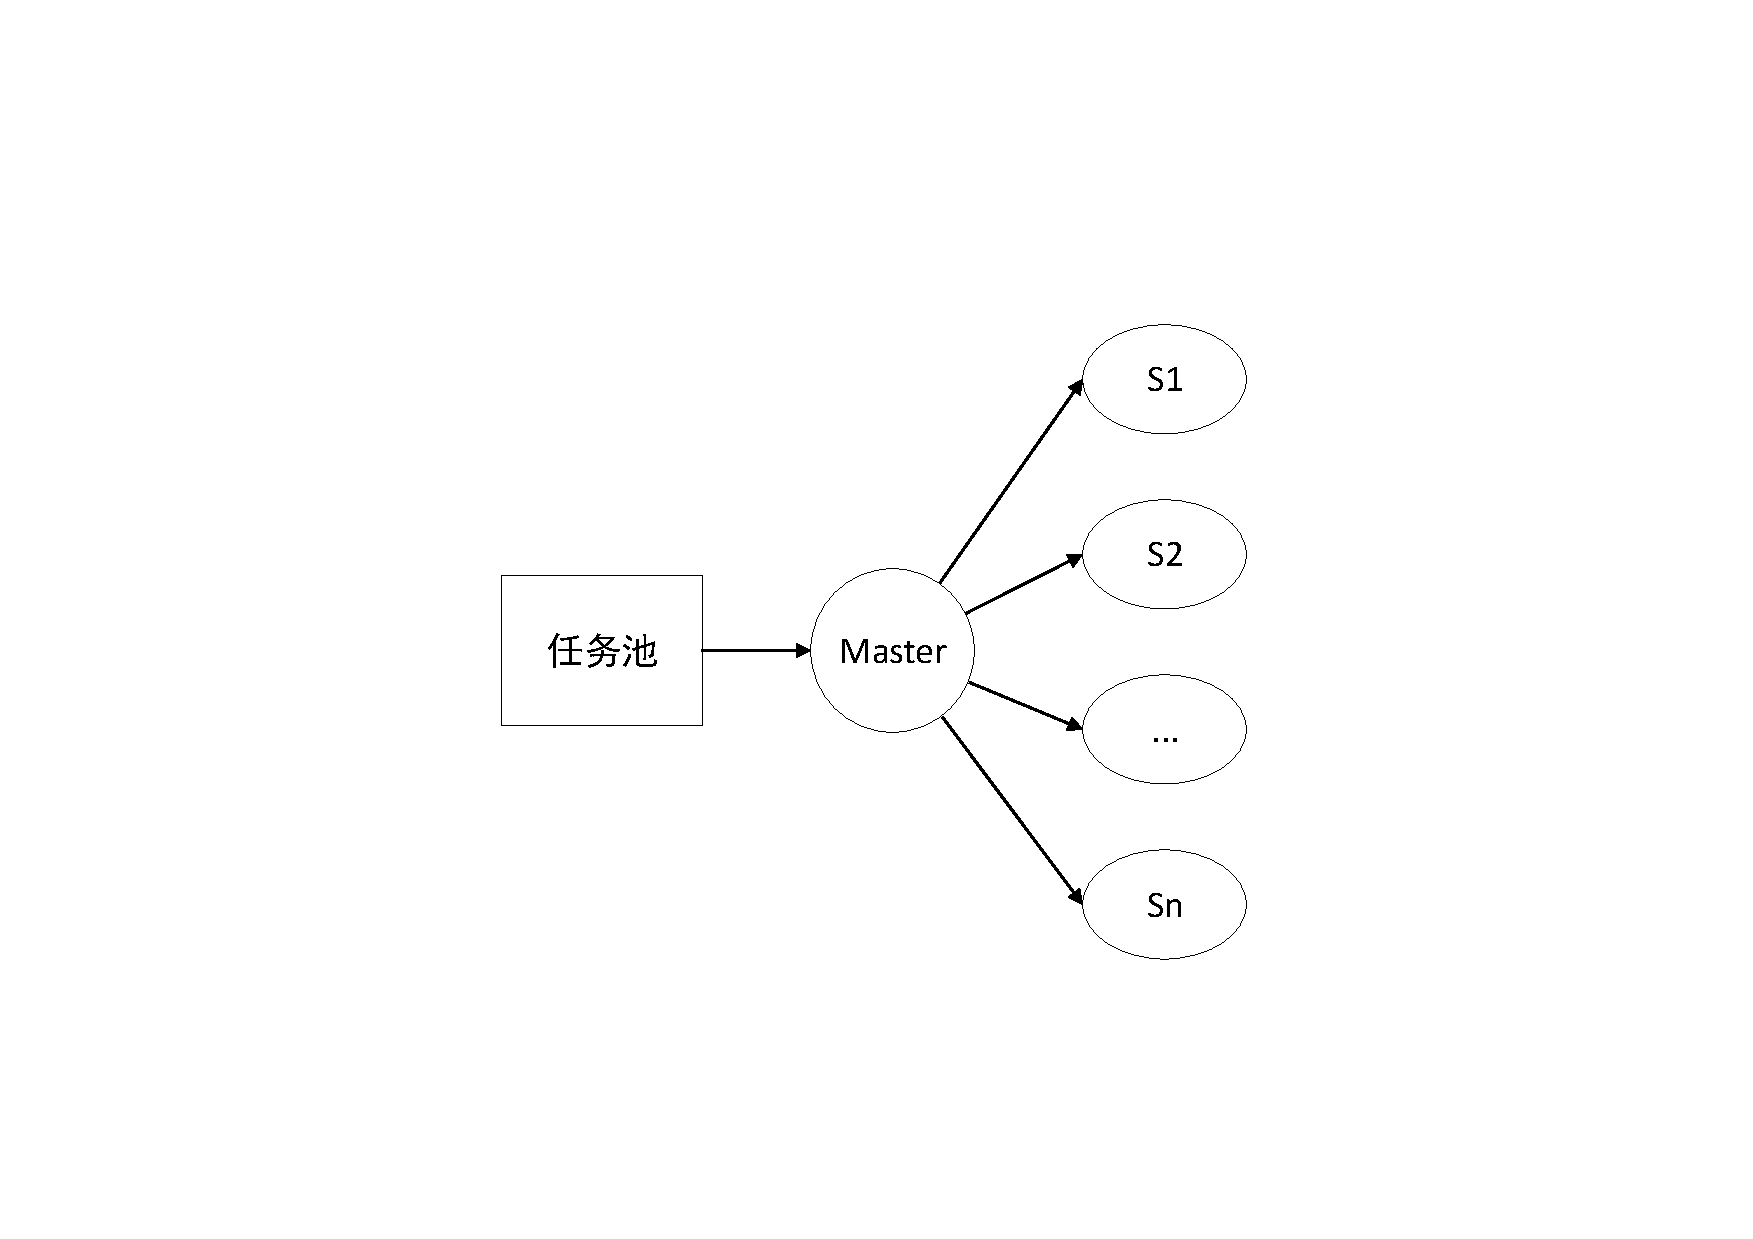
\includegraphics[width=0.6\textwidth]{fig/msp.pdf}
\caption{Master-Slave 调度模型}\label{msp}
\end{figure}

\subsection{PGSolve软件包的接口与实现}
根据上文所述的算法, 我们在 Maple 中实现了 PGSolve 软件包. PGSolve 软件包的核心接口是 GroupSolver 对象, 该对象实现了\reffig{PGSolve} 所述的功能. GroupSolver 的构造函数为:
\begin{verbatim}
GroupSolver(eqs,vrs,filter,{use_parallel});
\end{verbatim}
其中, 
\begin{compactitem}[\textbullet]
\item eqs 表示方程组;
\item vrs 表示需要求解的变量的集合;
\item filter 是一个用户自定义的函数, 对需要删除的解返回 true, 对需要保留的解返回 false;
\item 选项 \texttt{use\_parallel} 是可选的, 当用户指定这个选项时, GroupSolver 才会在求解时采用并行策略进行加速.
\end{compactitem}
当 GroupSolver 的构造完成时, 它会将 eqs, vrs, filter 作为成员变量进行存储, 同时初始化 SOLVED\D UNSOLVED 和 TIMEOUT 三个解的集合. 

当 GroupSolver 构造完成后, 用户就可以调用 GroupSolver:-agsolve(n,TL) 实现自动求解, 调用 GroupSolver:-pgsolve(n,TL) 实现分步求解. 其中, n表示分组求解的个数, 而TL表示单步求解的最长时间.  GroupSolver:-agsolve 对应实现了\reffig{PGSolve}的全部流程, 而GroupSolver:-pgsolve实现的则是从``SOL''节点开始到``是否为空?''的流程. 使用 agsolve 的优势在于整个求解流程自动完成, 缺点在于不能中途调整 n 和 TL. 而 pgsolve 则可以根据求解情况, 设置不同的 n 和 TL 进行求解. 

在Maple中, 并行可以分为基于 \texttt{Threads} 软件包的多线程并行和基于 \texttt{Grid} 软件包的多进程并行. 多线程并行可以进行资源共享, 但当多个线程同时访问一个资源时会存在线程安全的问题, 有可能导致程序出错. 因为 Maple 中许多重要的内置函数(如, solve)都不是线程安全的, 因此我们选择采用多进程并行. 多进程并行不存在资源共享的问题, 进程之间的交流靠通信实现. 尽管 \texttt{Grid} 软件包中有 \texttt{Map} 这样一个高级接口可以直接实现基于 Master-Slave 调度模型的并行过程, 但是为了控制整个计算过程的时长, 我们还是自行实现了一个 pmap 函数. 该函数的调用方式为 pmap(f,v,TL). 其中, f 是作用在 v 中每个元素上的函数, 而 TL 则是总的时间限制. GroupSolver 中的并行过程就是基于 pmap 函数实现的. 

\section{PGSolve在直接代数方法中的应用}
在微分方程的求解过程中, 许多方法最终都归结于代数方程组的求解. 包括齐次平衡方法\D 双曲正切方法和 Jacobi椭圆函数方法等, 最终都需要求解代数方程组. 不过这些方法最终的方程组规模都不大, 本文就不以它们举例了. 我们在\refchp{ch02}中, 基于简单 Hirota 方法求得了 NLEE 的孤子解\D 呼吸子解和LUMP 解. 其实, 我们也能通过直接代数方法来求解它们. 不过, 显然是\refchp{ch02}中的算法求解效率更高. 但是, 对于孤子解和LUMP解的相互作用解, 目前就只能利用直接代数方法进行求解. 由于求解该问题能够产生大规模的代数方程组, 我们就以该问题为例来展示 PGSolve 的作用, 同时测试 PGSolve 的有效性. 

\subsection{求 $n$-孤子和 1-LUMP 相互作用解的直接代数方法}
采用直接代数方法求 $n$-孤子和 1-LUMP 相互作用解的第一步和\refchp{ch02}中的简单 Hirota 方法一样, 都是利用 \Painleve{} 分析确定变换. 然后, 若自变量为$x_1,\cdots,x_m$, 则的假设形式为 
\begin{equation}
f_n=\sbrace{\xi_1+\eta_1}^2+\sbrace{\xi_2+\eta_2}^2+\sum_{i=1}^{2^n}\sbrace {q_i\prod_{k \in P_i}{\exp(\xi_{k+2})}}. \label{f-ns1l}
\end{equation}
其中, $P_i$ 是 $\bbrace{1,\cdots,n}$的全体子集中的第$i$个, 而
\begin{equation}
\xi_k=\sum_{j=1}^m{p_{j,k}x_j}.
\end{equation}
在\refeqn{f-ns1l}中, 前两个平方项的和构成了LUMP解的部分, 而最后一个求和项则是孤子解的部分. 在该假设形式中, 待定参数的集合为
\begin{equation}
    \bbrace{q_i|1\le i \le 2^n} \cup \bbrace{p_{j,k}|1\le j \le m, 1\le k \le n+2} \cup \bbrace{\eta_1,\eta_2}. 
\end{equation}

值得说明的是, 本文是在\refchp{ch02}中多孤子解的生成公式\refeqn{f-soliton-new}的基础上给出的\refeqn{f-ns1l}的. \refeqn{f-ns1l}的优点在于能够让高阶的解在某些参数取零时, 能够退化为相同形式的低阶解. 例如,
\begin{equation}
    f_1=\sbrace{\xi_1+\eta_1}^2+\sbrace{\xi_2+\eta_2}^2+q_1+q_2 \exp(\xi_3)
\end{equation}
在取$q_2=0$时, 可以退化为
\begin{equation}
    f_0=\sbrace{\xi_1+\eta_1}^2+\sbrace{\xi_2+\eta_2}^2+q_1.
\end{equation}
要想达到上述效果, 就需要对 $\bbrace{1,\cdots,n}$ 的全体子集进行合适的排序. 事实上, 按照\refalg{allsubset}生成的子集能够满足上述要求. 在\refalg{allsubset}中, 我们假设并集操作会保留元素的顺序. 

\begin{algorithm}
\caption{NS1L中的全体子集生成算法}\label{allsubset}
\Fn{$allsubset(n)$}{
    \lIf{$n=0$}{
        \Return{$\bbrace{\emptyset}$}
    }
    $X\gets allsubset(n-1)$\;
    \Return{$X \cup  \sbrace{\bigcup\limits_{v\in X}{v \cup \{n\}}}$}\;
}
\end{algorithm}

在确定了解的假设形式之后, 我们需要确定参数的约束条件. 按照相互作用解的实际意义, 需要满足:
\begin{compactenum}[(1)]
\item 孤子解的各个组成部分非零. 即$q_i\neq 0~(i=1,\cdots,2^n)$.
\item LUMP 的各个组成部分非零, 即$\xi_1\neq 0,\xi_2\neq 0$.
\item 多孤子解的各个孤子非零, 即$\xi_k\neq 0~(k=3,\cdots,n+2)$.
\item 孤子解部分和LUMP解部分解的维数不能退化, 即自变量的数量不能减少. 
\end{compactenum}

为了筛选出满足上述条件的解, 我们提出一个\emph{避免取值集合}的概念. 给定一个\emph{避免取值集合}$S$, 对于原方程组的一个解$t$ (是一个集合), 若存在$s\in S$, 满足$s\subseteq t$, 则$t$就不是我们想要的解. 而在我们的问题中, 
\begin{equation}
\begin{split}
    S&=\bbrace{\bbrace{q_i=0}|1\le i \le 2^n} \\ 
     &\cup \bbrace{\bbrace{p_{1,k}=0,\cdots,p_{m,k}=0}|1\le k \le n+2}  \\
     &\cup \bbrace{\bbrace{p_{j,1}=0,p_{j,2}=0}|1\le j \le m} \\ 
     &\cup \bbrace{\bbrace{p_{j,3}=0,\cdots,p_{j,n+2}=0}|1\le j \le m} . 
\end{split}
\end{equation}
式中第一个集合保证了孤子解的各个组成部分非零, 第二个集合保证了各个孤子非零以及LUMP解的各个部分非零, 第三个集合保证了LUMP解部分维数不退化, 而第四个集合保证了孤子解部分维数不退化.

\subsection{NS1L 和 PGSolve 软件包的应用实例}
基于上一节中的理论分析, 结合本文在 TwSolver 和 PGSolve 软件包上的工作, 我们开发了能够求解NLEE $n$-孤子和 1-LUMP 相互作用解的软件包 NS1L. 下面, 本文将以一个具体方程为例, 展示 NS1L 的调用方式, 测试 PGSolve 的求解性能. 

考虑(3+1)YTSF方程\CITEcaYTSF,
\begin{equation}
    3\,\alpha\,u_{{{\it yy}}}+4\,u_{{x}}u_{{{\it xz}}}+2\,u_{{{\it xx}}}u_{{z}}-4\,u_{{{\it tx}}}+u_{{{\it xxxz}}}=0. 
\end{equation}

求LUMP解, 演示一下调用过程, 解释一下参数含义. 最终得到4个解(考虑LUMP部分对偶关系则是3个解, 后期考虑实现以下这种等价的消除方法), 反正比 TwSolver 多, 对比一下, 到底有什么不同. 得到的结论应该是直接代数方法得到的解更一般. \todo{这里开始继续}

然后求1-孤子x1-LUMP 相互作用解, 这个时候提出直接求解和集成求解的区别, 突出一下本文公式很牛逼. 然后发现两种求解方式结果一样(3个, 但是应该是2个). 然后再画个图意思一下, 咦, 原来长得差不多啊. 不过不取全1这么特殊应该不至于张一样.

然后再提一下2孤子x1LUMP. 这个时候就能体现直接求解和继承求解的差别了. 最后, 可以挑3个解写个表达式画个图. 两个是只有一种方法有的解, 一个是共同的解. 

\section{小结}
PGSolve 真牛逼, 100小意思, 200中等意思. NS1L真牛逼, 继承求解真的骚. 
